\documentclass[english,russian, 10pt]{beamer}

\usepackage[T2A]{fontenc}
\usepackage[utf8]{inputenc} 
\usepackage[russian]{babel}
\usepackage[labelsep=period]{caption}
\usepackage{graphicx}
\usepackage{longtable}
\usepackage{amssymb}
\usepackage{amsmath}
\usepackage{makecell}
\usepackage{booktabs}
\usepackage{multirow}

\usepackage{colortbl}
\usepackage[table]{xcolor}
\usetheme{CambridgeUS}
\usecolortheme{beaver}

\usepackage{array}
\usepackage[export]{adjustbox}
\usepackage{tikz}
\usetikzlibrary{shapes.geometric, arrows.meta, positioning}

% \usepackage{ragged2e}
% \justifying
\setlength{\tabcolsep}{3pt}
\setbeamertemplate{caption}[numbered]
\setbeamertemplate{footline}[frame number]
\captionsetup[figure]{justification=centering}
\addto\captionsrussian{\renewcommand{\figurename}{Рисунок}}
\newcolumntype{C}[1]{>{\centering\let\newline\\\arraybackslash\hspace{0pt}}m{#1}}

\newcommand{\cel}{$\ ^\circ C$}
\newcommand{\cub}{\text{м}\textsuperscript{3}}

\usepackage{highlight}
\definecolor{low}{HTML}{ef3b2c} % the color for the highest value in your data  
\definecolor{mid}{HTML}{fff7f7}  % the color for the middle value in your data 
\definecolor{high}{HTML}{66FF66}  % the color for the lowest value in your data
\newcommand{\g}[1]{\gradientcelld{#1}{6}{10.5}{11.5}{low}{mid}{high}{70}}
\newcommand{\gc}[1]{\gradientcelld{#1}{7}{10.5}{11.8}{low}{mid}{high}{70}}


\title{Определение кода Голланда по результатам психометрических тестов личности на основе методов машинного обучения в условиях неполноты информации\\[0.5cm]}
\author{ГЛУШКОВ Егор Александрович\\[0.2cm]гр. 23.М04-мм, СПбГУ\\[0.2cm]
Научный руководитель: Абрамов~М.В.,\\[0.02cm]к.т.н., доцент кафедры информатики СПбГУ\\[0.2cm]
Консультант: Столярова В.Ф.,\\[0.02cm]старший преподаватель кафедры информатики СПбГУ}
\date{17 мая 2025}

\begin{document}

\begin{frame}[plain]
    \titlepage
\end{frame}


\begin{frame}{Введение}
    \begin{itemize}
        \item Значение корректного выбора профессионального пути
        \item Ресурсоёмкость традиционного глубинного интервью, дистанционные методы профориентации
        \item Модель RIASEC (код Голланда) и её ограничения: 
            \begin{itemize}
                \item шесть типов социально-профессиональной направленности личности
                \item различные вариации теста
                \item культурные и социо-экономические различия респондентов
                \item динамично меняющаяся ситуация на рынке профессий
            \end{itemize}
        \item Валидация результатов тестирования, связь с другими тестами, неполнота информации~--- восстановление результатов теста Голланда по альтернативным тестам
    \end{itemize}
\end{frame}


\begin{frame}{Постановка задачи}
    \emph{Цель}~--- разработать инструмент для автоматизации профориентации на основе определения кода Голланда по результатам психометрических тестов личности с использованием методов машинного обучения\\[0.3cm]
    \emph{Задачи}:
    \begin{enumerate}
        \item Изучить и систематизировать существующие подходы к определению кода Голланда на основе психометрических данных
        \item Реализовать и сравнить методы машинного обучения для предсказания кодов Голланда
        \item Разработать алгоритмы восстановления результатов психометрических тестов в случае неполноты данных
        \item Создать прототип инструмента для определения профориентационных предпочтений
    \end{enumerate}
\end{frame}


\begin{frame}{Постановка задачи [2]}
    \begin{itemize}
        \item \emph{Новизна результатов исследования}: использование комбинации различных психометрических тестов для предсказания кода Голланда
        \item \emph{Теоретическая значимость}: создание новых моделей машинного обучения для определения взаимосвязи психометрических тестов и кода Голланда
        \item \emph{Практическая значимость}: реализация прототипа программного модуля автоматизации оценки профессиональной направленности по психологическому профилю личности
    \end{itemize}
\end{frame}


\begin{frame}{Обзор. Психометрические  тесты личности}
    \begin{itemize}
    \item Психологические тесты личности (количество факторов):
        \begin{enumerate}
            \item Модель Голланда RIASEC (6)
            \item Опросник Леонгарда-Шмишека (10)
            \item Личностный опросник Айзенка (4)
            \item 16-факторный опросник Кеттелла (16)
            \item Пятифакторный опросник личности («Большая пятерка»; 5)
            \item Ценностный опросник Шварца (20)
        \end{enumerate}
    \item Цель тестирования~--- отразить некоторые черты личности человека в удобном целочисленном формате
    \item Модель Голланда RIASEC – 6 типов личностей, с которыми соотнесены наборы профессий:
        \begin{itemize}
            \item[-] реалистический (Realistic, R)
            \item[-] исследовательский (Investigative, I)
            \item[-] артистический (Artistic, A)
            \item[-] социальный (Social, S)
            \item[-] предприимчивый (Enterprising, E)
            \item[-] традиционный (Conventional, C)
        \end{itemize}
    \end{itemize}
\end{frame}


\begin{frame}{Пример входных данных}
    \begingroup
      \fontsize{7pt}{9pt}\selectfont
        \begin{table}[ht]
            \centering
            \caption{Пример данных психометрических тестов}
            \label{tab:input_test_data}
            \begin{tabular}{l|rrrr rr|rrrrrr}
                \toprule
                & \multicolumn{3}{c}{Большая Пятёрка}
                & \multicolumn{1}{c}{\dots}
                & \multicolumn{2}{c}{Леонгард}
                & \multicolumn{6}{c}{Голланд} \\
                \cmidrule(lr){2-4} \cmidrule(lr){5-5} \cmidrule(lr){6-7} \cmidrule(lr){8-13}
                id 
                & BF\_1 & BF\_2 & BF\_3 
                & \dots 
                & LN\_9 & LN\_10 
                & HL\_1 & HL\_2 & HL\_3 & HL\_4 & HL\_5 & HL\_6 \\
                \midrule
                1 & 39 & 66 & 33 & \dots &  3 & 12  &  8 &  8 &  6 &  8 &  1 & 11 \\
                2 & 45 & 46 & 73 & \dots & 12 &  6  &  3 &  7 &  7 &  8 & 10 &  7 \\
                3 & 34 & 41 & 56 & \dots & 18 & 12  & 10 & 10 &  3 & 11 &  7 &  1 \\
                4 & 49 & 47 & 50 & \dots & 15 & 24  &  6 &  4 &  8 &  6 &  7 & 11 \\
                5 & 48 & 42 & 53 & \dots & 12 &  6  &  6 &  7 &  8 &  7 & 10 &  4 \\
                \bottomrule
            \end{tabular}
        \end{table}
    \endgroup

    \begin{itemize}
        \item VK Mini Apps «Психологические тесты»
        \item Анонимизированные данные 1278 пользователей: 339~-- полные, 939~-- заполнены данные по 4 или 5 тестам
        \item Обработка данных: валидация, заполнение пропусков, стандартизация, уменьшение размерности PCA
    \end{itemize}
\end{frame}


\begin{frame}{Методы решения}
    Методы решения задачи по определению кода Голланда:
    \begin{itemize}
        \item Многоцелевая регрессия
        \item Классификация
        \item Ранжирование
    \end{itemize}
    \vspace{0.3em}
    Реализация вычислительного эксперимента:
    \begin{itemize}
        \item R (data.table, R6Class), Python (PyTorch)
        \item Стенд: R Shiny
    \end{itemize}
\end{frame}


\begin{frame}{Регрессия. Подходы}
    \begin{figure}[h]
        \centering
        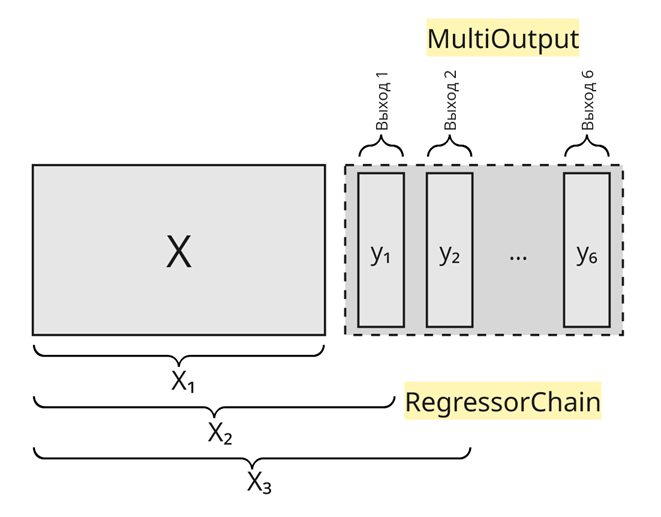
\includegraphics[width=0.7\textwidth]{images/regr.png}
        \caption{Подходы к решению задачи многоцелевой регрессии}
        \label{fig:MO_regr}
    \end{figure}
\end{frame}


\begin{frame}{Регрессия. Метрики качества}
  \begin{itemize}
    \item Усреднённая среднеквадратичная ошибка (RMSE)
    \item Усреднённый C‑индекс: мера согласованности (чем больше, тем более схожи профили личности)

  \vspace{0.3em}
  \item C‑индекс для трёхбуквенных кодов (верхних триад):
  \[
    C = 3\, (X_1, Y_1) + 2\, (X_2, Y_2) + 1\, (X_3, Y_3),
  \]
  где $\{X_i\}$ и $\{Y_i\}$ — первые три позиции кодов Голланда, их позиции в замкнутой цепочке (шестиугольнике) R-I-A-S-E-C:
  \[
    (X_i, Y_i) =
    \begin{cases}
      3, & \text{если $X_i = Y_i$,}\\
      2, & \text{если $X_i$ и $Y_i$ -- соседние позиции,}\\
      1, & \text{если $X_i$ и $Y_i$ -- позиции через один код,}\\
      0, & \text{если $X_i$ и $Y_i$ -- противоположны}
    \end{cases}
  \]

  \item Пример: 
    \(\displaystyle 
      C\bigl([6,10,4,5,8,9],\,[6,6,7,9,6,8]\bigr)
      =\)
    \[
      C(\mathrm{ICE},\,\mathrm{SCA})
      =3\cdot1 + 2\cdot3 + 1\cdot1
      =10
    \]
    \end{itemize}
\end{frame}


\begin{frame}{Регрессия. Результаты (C-индекс)}
  \begingroup
    \fontsize{8pt}{9pt}\selectfont
    \begin{table}[ht]
      \centering
      \caption{Сравнение моделей по метрике C‑индекс}
      \label{tab:model-comparison}
        \setlength{\tabcolsep}{2pt}
        \begin{tabular*}{0.9\textwidth}{@{\extracolsep{\fill}} 
          >{\raggedright\arraybackslash}p{4.85cm}  
          | *{4}{>{\centering\arraybackslash}p{1.25cm}}
        @{}}
      \toprule
          \textbf{Модель} 
            & \textbf{МО}      
            & \textbf{МО PCA}   
            & \textbf{Chain}   
            & \textbf{Chain PCA} \\
        \midrule
        Регрессия Lasso (L1)      & \g{11.175} & \g{10.887} & \g{11.175} & \g{11.150} \\
        ExtraTrees                & \g{10.700} & \g{11.100} & \g{10.625} & \g{10.825} \\
        Регрессия Ridge (L2)      & \g{10.988} & \g{10.537} & \g{11.062} & \g{10.412} \\

        \arrayrulecolor[gray]{0.8}
        \specialrule{0.75pt}{0pt}{0pt}
        \arrayrulecolor{black}
        
        Метод опорных векторов    & \g{10.713} & \g{10.950} & \g{10.713} & \g{10.950} \\
        Пошаговая регрессия       & \g{10.600} & \g{10.900} & \g{10.600} & \g{10.900} \\
        CatBoost                  & \g{10.688} & \g{10.812} & \g{10.688} & \g{10.812} \\
        Random Forest             & \g{10.625} & \g{10.475} & \g{10.812} & \g{10.588} \\
        Линейная регрессия (OLS)  & \g{10.688} & \g{10.800} & \g{10.688} & \g{10.800} \\
        LightGBM                  & \g{10.750} & \g{10.425} & \g{10.750} & \g{10.425} \\
        kNN                       & \g{10.525} & \g{10.400} & \g{10.525} & \g{10.400} \\
        XGBoost                   & \g{9.162}  & \g{9.725}  & \g{9.162}  & \g{9.725}  \\
        Constant baseline         & \g{9.000}  & \g{9.000}  & \g{9.000}  & \g{9.000}  \\
        \midrule
        TabPFN                    & \g{10.562} &            &            &            \\
        MLP (BatchNorm, DropOut, регул-я) & \g{10.462} &    &            &            \\
        MLP                       & \g{10.275} &            &            &            \\
        \bottomrule
      \end{tabular*}
      \vspace{0.75em}
      \begin{minipage}{0.9\textwidth}
        \scriptsize
        \hspace{1em}\textit{* MO~--- Multioutput, PCA~--- метод главных компонент (уменьшение размерности)}
      \end{minipage}
    \end{table}
  \endgroup
\end{frame}


\newcommand{\grmse}[1]{\gradientcelld{#1}{2.0}{2.1}{2.7}{high}{mid}{low}{70}}

\begin{frame}{Регрессия. Результаты (RMSE)}
  \begingroup
    \fontsize{8pt}{9pt}\selectfont
    \begin{table}[ht]
      \centering
      \caption{Сравнение моделей по метрике RMSE}
      \label{tab:rmse-comparison}
        \setlength{\tabcolsep}{2pt}
        \begin{tabular*}{0.9\textwidth}{@{\extracolsep{\fill}} 
          >{\raggedright\arraybackslash}p{4.85cm}  
          | *{4}{>{\centering\arraybackslash}p{1.25cm}}
        @{}}
      \toprule
          \textbf{Модель} 
            & \textbf{МО}      
            & \textbf{МО PCA}   
            & \textbf{Chain}   
            & \textbf{Chain PCA} \\
        \midrule
        Регрессия Lasso (L1)      & \grmse{2.018} & \grmse{2.036} & \grmse{2.018} & \grmse{2.030} \\
        Линейная регрессия (OLS)  & \grmse{2.155} & \grmse{2.019} & \grmse{2.155} & \grmse{2.019} \\
        Регрессия Ridge (L2)      & \grmse{2.025} & \grmse{2.037} & \grmse{2.028} & \grmse{2.044} \\
        Пошаговая регрессия       & \grmse{2.094} & \grmse{2.027} & \grmse{2.094} & \grmse{2.027} \\
        CatBoost                  & \grmse{2.044} & \grmse{2.096} & \grmse{2.044} & \grmse{2.096} \\
        Random Forest             & \grmse{2.069} & \grmse{2.131} & \grmse{2.070} & \grmse{2.133} \\
        LightGBM                  & \grmse{2.074} & \grmse{2.128} & \grmse{2.074} & \grmse{2.128} \\
        Метод опорных векторов (SVR) & \grmse{2.100} & \grmse{2.101} & \grmse{2.100} & \grmse{2.101} \\
        ExtraTrees                & \grmse{2.100} & \grmse{2.150} & \grmse{2.112} & \grmse{2.152} \\
        kNN                       & \grmse{2.162} & \grmse{2.151} & \grmse{2.162} & \grmse{2.151} \\
        Constant baseline         & \grmse{2.308} & \grmse{2.308} & \grmse{2.308} & \grmse{2.308} \\
        XGBoost                   & \grmse{2.317} & \grmse{2.314} & \grmse{2.317} & \grmse{2.314} \\
        \midrule
        TabPFN                    & \grmse{2.056} &            &            &            \\
        MLP (BatchNorm, DropOut, регул-я) & \grmse{2.143} &            &            &            \\
        MLP                       & \grmse{2.442} &            &            &            \\
        \bottomrule
      \end{tabular*}
      \vspace{0.75em}
      \begin{minipage}{0.9\textwidth}
        \scriptsize
        \hspace{1em}\textit{* MO~--- Multioutput, PCA~--- метод главных компонент (уменьшение размерности)}
      \end{minipage}
    \end{table}
  \endgroup
\end{frame}



\begin{frame}{Анализ важности признаков}
  \begingroup
    \fontsize{8pt}{9pt}\selectfont
    \begin{table}[ht]
      \centering
      \caption{Важность признаков модели Random Forest}
      \label{tab:feature-importance}
      \begin{tabular*}{0.95\textwidth}{@{\extracolsep{\fill}} c|p{5cm} c c @{}}
        \toprule
        Код признака 
          & Наименование признака 
          & Важность (\%) 
          & Накоплено (\%) \\
        \midrule
        CT\_1   & Открытость – Замкнутость                & 15.5 & 15.5 \\
        CT\_7   & Чувственность – Твердость               & 15.5 & 31.0 \\
        SC\_19  & Гедонизм – индив. приоритет             & 4.2  & 35.2 \\
        EY\_1   & Экстраверсия                            & 4.0  & 39.2 \\
        CT\_4   & Беспечность – Озабоченность             & 3.6  & 42.8 \\
        SC\_3   & Власть – нормат. идеал                  & 3.4  & 46.2 \\
        LN\_3   & Циклотимность                           & 3.3  & 49.5 \\
        BF\_3   & Самоконтроль – импульсивность           & 2.5  & 52.0 \\
        BF\_4   & Эмоц. устойчивость – неустойчивость     & 2.5  & 54.5 \\
        \bottomrule
      \end{tabular*}
    \end{table}
  \endgroup
\end{frame}


\begin{frame}{Регрессия. Ансамблевые модели}
  \begin{itemize}
    \item \textbf{Ансамблевые модели:}
      \begin{itemize}
        \item Стекинг
        \item Линейный блендинг (взвешенное ансамблирование)
      \end{itemize}
    \vspace{0.3em}
    \item Методы подбора весов для блендинга:
      \begin{itemize}
        \item Равные веса всех моделей
        \item Вектор Шэпли
        \item Частичный перебор по сетке
        \item Квадратичная оптимизация (QP)
        \item Генетический алгоритм (GA)
        \item Метод роя частиц (PSO)
        \item Координатный спуск
      \end{itemize}
    \vspace{0.3em} 
    \item Опционально использовалось уменьшение размерности (PCA)
  \end{itemize}
\end{frame}

\renewcommand{\gc}[1]{\gradientcelld{#1}{9}{11.1}{11.8}{low}{mid}{high}{70}}

\begin{frame}{Регрессия. Ансамблирование регрессоров -- результаты}
  \begingroup
    \fontsize{8pt}{9pt}\selectfont

    \setlength{\abovecaptionskip}{3pt}
    \setlength{\belowcaptionskip}{1.5pt}
    
    \begin{table}[ht]
      \centering
      \caption{Сравнение методов подбора весов ансамбля регрессионных моделей}
      \label{tab:ensemble-weights}
      \begin{tabular*}{0.95\textwidth}{@{\extracolsep{\fill}} 
        l|
        *{4}{>{\centering\arraybackslash}p{1.3cm}}
      @{}}
        \toprule
        Метод подбора весов 
          & MO 
          & MO избр.
          & Chain 
          & Chain избр. \\
        \midrule
        Равные веса всех моделей       & \gc{11.063} & \gc{11.088} & \gc{11.050} & \gc{11.013} \\
        Вектор Шэпли (Shap)            & \gc{11.050} & \gc{11.138} & \gc{11.138} & \gc{11.050} \\
        Частичный перебор по сетке     & \gc{11.550} & \gc{11.388} & \gc{11.538} & \gc{11.325} \\
        Квадратичная оптимизация (QP)  & \gc{10.588} & \gc{10.463} & \gc{10.738} & \gc{10.813} \\
        Генетический алгоритм (GA)     & \gc{11.500} & \gc{11.550} & \gc{11.300} & \gc{11.563} \\
        Метод роя частиц (PSO)         & \gc{11.600} & \gc{11.663} & \gc{11.613} & \gc{11.613} \\
        Координатный спуск             & \gc{11.188} & \gc{11.225} & \gc{11.288} & \gc{11.413} \\
        \midrule
        % новые строки
        Линейные регрессии с регуляризацией 
          & \multicolumn{2}{c}{Линейная регрессия} 
          & \multicolumn{2}{c}{\gc{10.887}} \\
        Lasso, Ridge, LightGBM, CatBoost, RF 
          & \multicolumn{2}{c}{Линейная регрессия} 
          & \multicolumn{2}{c}{\gc{10.688}} \\
        \bottomrule
      \end{tabular*}
      \vspace{0.5em}
      \begin{minipage}{0.9\textwidth}
          \scriptsize
          \textit{* MO~--- Multioutput, 'избр.'~--- подбор весов только для топ‑5 моделей согласно C‑индексу}
      \end{minipage}
    \end{table}

    \vspace{-1.2em}
    \setlength{\abovecaptionskip}{3pt}
    \setlength{\belowcaptionskip}{1.5pt}

    \begin{table}[ht]
      \centering
      \caption{Весовые коэффициенты моделей и C‑индекс}
      \label{tab:pso-weights}
      \begingroup
        \fontsize{8pt}{9pt}\selectfont
        \begin{tabular*}{0.95\textwidth}{@{\extracolsep{\fill}} 
          l|*{4}{c}|>{\centering\arraybackslash}p{1.15cm}
        @{}}
          \toprule
          Метод подбора 
            & \multicolumn{4}{c|}{Веса моделей} 
            & C‑индекс \\
          \cmidrule(lr){2-5}
          весов 
            & Lasso L1
            & Пошаговая регр. 
            & CatBoost 
            & ExtraTrees 
            &  \\
          \midrule
          PSO & 0.432 & 0.327 & 0.150 & 0.091 & 11.663 \\
          \bottomrule
        \end{tabular*}
      \endgroup
    \end{table}
    
  \endgroup
\end{frame}


\begin{frame}{Распределение C-индекса предсказаний}
    \begin{figure}
        \centering
        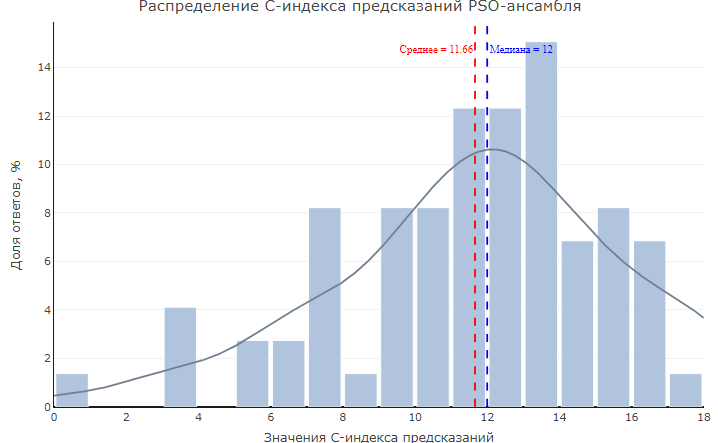
\includegraphics[width=0.8\linewidth]{images/distr_cind.png}
        \caption{Распределение C-индекса предсказаний PSO-модели}
        \label{fig:distr_cind}
    \end{figure}
\end{frame}


\begin{frame}{Классификация. Подходы}
  \begingroup
    \fontsize{8pt}{9pt}\selectfont
    \begin{table}[ht]
      \centering
      \caption{Подходы к классификации}
      \label{tab:classification-types}
      \begin{tabular*}{0.95\textwidth}{@{\,}
        >{\centering\arraybackslash}p{2.75cm} |
        >{\centering\arraybackslash}p{2.75cm} |
        >{\centering\arraybackslash}p{2.75cm} |
        c @{}}
        \toprule
        \textbf{Тип классификации}
          & \textbf{Модель}
          & \textbf{Значение}
          & \textbf{Пример} \\
        \midrule
        Многоклассовая (multiclass)
          & 1 классификатор на 6 классов
          & 3 кода из 1 буквы
          & R, S, E \\
        \addlinespace[0.25em] \hline \addlinespace[0.25em]
        Многометочная (multilabel)
          & 6 бинарных классификаторов
          & Булевый вектор из 6 элементов с 3 \texttt{True}
          & [T, F, F, T, T, F] \\
        \addlinespace[0.5em] \hline \addlinespace[0.25em]
        Label powerset
          & 1 классификатор на 20 классов (порядок не важен)
          & 3‑буквенный код
          & RSE \\
        \bottomrule
      \end{tabular*}
    \end{table}
  \endgroup
   \begin{itemize}
        \item Верхняя триада~--- три наиболее значимых кода
        \item Метрики: Top-K accuracy, C-индекс
        \item Опционально уменьшение размерности (PCA)
    \end{itemize}
\end{frame}


\begin{frame}{Классификация. Сравнение подходов}
  \begingroup
    \fontsize{8pt}{9pt}\selectfont
    \setlength{\tabcolsep}{3pt}
    \begin{table}[ht]
      \centering
      \caption{Сравнение подходов к классификации (Top-K accuracy)}
      \label{tab:classification-comparison}
      \begin{tabular*}{0.95\textwidth}{@{\extracolsep{\fill}} 
        p{2.5cm}|
        *{3}{>{\centering\arraybackslash}p{0.7cm}}|
        *{3}{>{\centering\arraybackslash}p{0.7cm}}|
        *{3}{>{\centering\arraybackslash}p{0.7cm}}
      @{}}
        \toprule
        \textbf{Модель}
          & \multicolumn{3}{c|}{\textbf{Multiclass}}
          & \multicolumn{3}{c|}{\textbf{Multilabel}}
          & \multicolumn{3}{c}{\textbf{Label Powerset}} \\
        \cmidrule(lr){2-4}\cmidrule(lr){5-7}\cmidrule(lr){8-10}
          & Top‑1 & Top‑2 & Top‑3 
          & Top‑1 & Top‑2 & Top‑3 
          & Top‑1 & Top‑2 & Top‑3 \\
        \midrule
        kNN                     & 0.988 & 0.713 & 0.125 & 1.000 & 0.763 & 0.113 & 0.975 & 0.650 & 0.175 \\
        Логист. L1-регр.      & 1.000 & 0.700 & 0.163 & 1.000 & 0.700 & 0.163 & 0.988 & 0.638 & 0.100 \\
        XGBoost                 & 1.000 & 0.700 & 0.113 & 0.975 & 0.675 & 0.100 & 0.963 & 0.625 & 0.113 \\
        Логист. L2-регр.      & 1.000 & 0.700 & 0.150 & 0.988 & 0.700 & 0.213 & 0.988 & 0.675 & 0.088 \\
        Наивный Байес           & 0.975 & 0.700 & 0.150 & 0.988 & 0.700 & 0.150 & 0.988 & 0.688 & 0.163 \\
        ExtraTrees              & 0.996 & 0.725 & 0.150 & 1.000 & 0.775 & 0.146 & 0.975 & 0.688 & 0.200 \\
        SVM                     & 1.000 & 0.742 & 0.146 & 1.000 & 0.721 & 0.138 & 0.975 & 0.675 & 0.213 \\
        Random Forest           & 1.000 & 0.742 & 0.158 & 0.996 & 0.738 & 0.146 & 0.988 & 0.638 & 0.225 \\
        CatBoost                & 0.988 & 0.788 & 0.113 & 0.988 & 0.788 & 0.113 & 0.988 & 0.700 & 0.163 \\
        LightGBM                & 0.975 & 0.563 & 0.050 & 0.975 & 0.700 & 0.100 & 0.950 & 0.525 & 0.050 \\

        \bottomrule
      \end{tabular*}
    \end{table}
  \endgroup
\end{frame}


\renewcommand{\gc}[1]{\gradientcelld{#1}{7}{10.35}{11.3}{low}{mid}{high}{70}}

\begin{frame}{Классификация. Сравнение моделей}
  \begingroup
    \fontsize{8pt}{9pt}\selectfont
    \setlength{\tabcolsep}{0pt}
    \begin{table}[ht]
      \centering
      \caption{Сравнение классификаторов}
      \label{tab:classification-models}
      \begin{tabular*}{0.95\textwidth}{@{\extracolsep{\fill}}
        >{\raggedright\arraybackslash}p{3.5cm}  % Классификатор
        >{\centering\arraybackslash}p{1.2cm}     % Подход
        >{\centering\arraybackslash}p{1.7cm}     % C‑индекс
        *{3}{>{\centering\arraybackslash}p{1.1cm}} % Top‑1,2,3
      @{}}
        \toprule
        \textbf{Классификатор}
          & \textbf{Подход}
          & \textbf{C‑индекс}
          & \textbf{Top‑1}
          & \textbf{Top‑2}
          & \textbf{Top‑3} \\
        \midrule
        kNN                            & Multilabel & \gc{10.838} & 1.000 & 0.763 & 0.113 \\
        Логистическая регр. (L1)       & Multiclass & \gc{10.663} & 1.000 & 0.700 & 0.163 \\
        XGBoost                        & Multiclass & \gc{10.638} & 1.000 & 0.700 & 0.113 \\
        Логистическая регр. (L2)       & Multiclass & \gc{10.500} & 1.000 & 0.700 & 0.150 \\
        Наивный Байес                  & Multilabel & \gc{10.350} & 0.988 & 0.700 & 0.150 \\
        ExtraTrees                     & Multilabel & \gc{10.013} & 1.000 & 0.775 & 0.146 \\
        SVM                            & Multilabel & \gc{9.875}  & 1.000 & 0.721 & 0.138 \\
        Random Forest                  & Multilabel & \gc{9.800}  & 0.996 & 0.738 & 0.146 \\
        CatBoost                       & Multilabel & \gc{9.775}  & 0.988 & 0.788 & 0.113 \\
        LightGBM                       & Multilabel & \gc{9.313}  & 0.975 & 0.700 & 0.100 \\
        Baseline (случайный)           & –          & \gc{9.000}  & 0.950 & 0.500 & 0.050 \\
        \bottomrule
      \end{tabular*}
    \end{table}
  \endgroup
\end{frame}


\renewcommand{\gc}[1]{\gradientcelld{#1}{8}{10.8}{11.7}{low}{mid}{high}{70}}

\begin{frame}{Ансамблирование классификаторов -- результаты}
  \begingroup
    \fontsize{8pt}{9pt}\selectfont
    \setlength{\tabcolsep}{2pt}
    \begin{table}[ht]
      \centering
      \caption{Сравнение методов подбора весов ансамбля классификаторов}
      \label{tab:ensemble-results}
      \begin{tabular*}{0.95\textwidth}{@{\extracolsep{\fill}}
        >{\raggedright\arraybackslash}p{4.5cm} 
        *{3}{>{\centering\arraybackslash}p{2.1cm}}
      @{}}
        \toprule
        \textbf{Метод подбора весов}
          & \textbf{Multiclass}
          & \textbf{Multilabel}
          & \textbf{Label Powerset} \\
        \midrule
        Равные веса всех моделей      & \gc{10.663} & \gc{10.888} & \gc{10.563} \\
        Вектор Шэпли (Shap)           & \gc{10.563} & \gc{11.038} & \gc{10.525} \\
        Частичный перебор по сетке    & \gc{11.213} & \gc{11.488} & \gc{11.525} \\
        Квадратичная оптимизация (QP) & \gc{10.488} & \gc{10.638} & \gc{10.650} \\
        Генетический алгоритм (GA)    & \gc{11.263} & \gc{11.313} & \gc{11.213} \\
        Метод роя частиц (PSO)        & \gc{11.263} & \gc{11.625} & \gc{11.525} \\
        Координатный спуск             & \gc{11.200} & \gc{11.275} & \gc{10.425} \\
        \bottomrule
      \end{tabular*}
    \end{table}

    \vspace{-1.2em}
    \setlength{\abovecaptionskip}{3pt}
    \setlength{\belowcaptionskip}{1.5pt}

    \begin{table}[ht]
      \centering
      \caption{Весовые коэффициенты моделей и C‑индекс}
      \label{tab:pso-weights-full}
      \begingroup
        \fontsize{7pt}{9pt}\selectfont
        \begin{tabular*}{0.95\textwidth}{@{\extracolsep{\fill}} 
          l|*{8}{c}|>{\centering\arraybackslash}p{1.1cm}
        @{}}
          \toprule
          Метод подбора 
            & \multicolumn{8}{c|}{Веса моделей} 
            & C‑инд \\
          \cmidrule(lr){2-9}
          весов 
            & kNN
            & SVM
            & Logit L1
            & XGBoost
            & LightGBM
            & NaiveBayes
            & ExtraTrees
            & RF
            & \\
          \midrule
          PSO 
            & 0.291 
            & 0.164 
            & 0.191 
            & 0.183 
            & 0.151 
            & 0.009 
            & 0.007 
            & 0.004 
            & 11.625 \\
          \bottomrule
        \end{tabular*}
      \endgroup
    \end{table}

  \endgroup
\end{frame}


\renewcommand{\gc}[1]{\gradientcelld{#1}{7}{9.6}{11.5}{low}{mid}{high}{70}}
\newcommand{\gndcg}[1]{\gradientcelld{#1}{0.25}{0.54}{0.7}{low}{mid}{high}{70}}

\begin{frame}{Ранжирование}
   \begin{itemize}
        \item Списочное ранжирование~--- Listwise Learn-to-Rank
        \item Задание скоринговой функции (MLP, Deep and Cross Network, Transformer) и функции потерь для списков (NDCG, ApproxNDCG, LambdaRank, ListNet@k)
    \end{itemize}

    \begin{table}[ht]
      \centering
      \caption{Сравнение моделей ранжирования}
      \label{tab:loss-functions}
      \begingroup
        \fontsize{8pt}{9pt}\selectfont
        \setlength{\tabcolsep}{2pt}
        \begin{tabular*}{0.95\textwidth}{@{\extracolsep{\fill}} 
          >{\raggedright\arraybackslash}p{2cm}  % Функция потерь
          | *{3}{>{\centering\arraybackslash}p{1.35cm}}  % C‑индекс
          | *{3}{>{\centering\arraybackslash}p{1.35cm}}  % NDCG@3
        }
          \toprule
            \textbf{Функция}  
              & \multicolumn{3}{c|}{\textbf{C‑индекс}} 
              & \multicolumn{3}{c}{\textbf{NDCG@3}} \\
            \cmidrule(lr){2-4} \cmidrule(lr){5-7}
            \textbf{потерь}
            & Deep and Cross 
            & Listwise Transformer 
            & MLP 
            & Deep and Cross 
            & Listwise Transformer 
            & MLP \\
          \midrule
          ApproxNDCG   & \gc{10.025} & \gc{8.888}  & \gc{9.150}  & \gndcg{0.539} & \gndcg{0.439} & \gndcg{0.388} \\
          LambdaRank   & \gc{9.963}  & \gc{9.675}  & \gc{9.650}  & \gndcg{0.527} & \gndcg{0.489} & \gndcg{0.543} \\
          ListNet@1    & \gc{9.650}  & \gc{10.325} & \gc{10.438} & \gndcg{0.504} & \gndcg{0.628} & \gndcg{0.653} \\
          ListNet@3    & \gc{9.450}  & \gc{9.950}  & \gc{10.788} & \gndcg{0.458} & \gndcg{0.622} & \gndcg{0.638} \\
          \bottomrule
        \end{tabular*}
      \endgroup
    \end{table}
\end{frame}


\renewcommand{\gc}[1]{\gradientcelld{#1}{7}{9.6}{10.9}{low}{mid}{high}{70}}

\begin{frame}{Восстановление пропусков в случае неполноты данных}
  \begingroup
    \fontsize{8pt}{9pt}\selectfont
    \setlength{\tabcolsep}{3pt}
    \begin{table}[ht]
      \centering
      \caption{Восстановление значений незаполненных психометрических тестов}
      \label{tab:imputation-comparison}
      \begin{tabular*}{0.95\textwidth}{@{\extracolsep{\fill}} 
        >{\raggedright\arraybackslash}p{3cm} 
        *{4}{>{\centering\arraybackslash}p{1.88cm}}
      @{}}
        \toprule
        \textbf{Модель-регрессор}
          & \textbf{MICE}
          & \textbf{Matrix Soft Impute}
          & \textbf{Маски}
          & \textbf{Линейный блендинг} \\
        \midrule
        Регрессия Lasso (L1)              & \gc{9.191} & \gc{10.090} & \gc{9.998} & \gc{9.866} \\
        Пошаговая регрессия               & \gc{9.608} & \gc{9.754}  & \gc{9.978} & \gc{10.082}\\
        Линейная регр. (OLS)              & \gc{9.407} & \gc{9.612}  & \gc{9.876} & \gc{10.012}\\
        Регрессия Ridge (L2)              & \gc{9.442} & \gc{9.733}  & \gc{9.868} & \gc{9.933} \\
        ExtraTrees                        & \gc{9.101} & \gc{9.627}  & \gc{9.870} & \gc{9.808} \\
        Метод опорных векторов (SVR)      & \gc{9.221} & \gc{9.622}  & \gc{9.864} & \gc{9.760} \\
        CatBoost                          & \gc{9.131} & \gc{9.766}  & \gc{9.835} & \gc{9.461} \\
        kNN                               & \gc{9.372} & \gc{9.486}  & \gc{9.830} & \gc{9.377} \\
        Random Forest                     & \gc{9.518} & \gc{9.710}  & \gc{9.819} & \gc{9.712} \\
        LightGBM                          & \gc{9.372} & \gc{9.678}  & \gc{9.686} & \gc{9.594} \\
        XGBoost                           & \gc{8.769} & \gc{9.571}  & \gc{9.267} & \gc{9.614} \\
        Constant baseline                 & \gc{9.000} & \gc{9.000}  & \gc{9.000} & \gc{9.000} \\
        \bottomrule
      \end{tabular*}
    \end{table}
  \endgroup
\end{frame}


\renewcommand{\gc}[1]{\gradientcelld{#1}{7}{10}{11.7}{low}{mid}{high}{60}}

\begin{frame}{Сводные результаты по типам задач}
  \begingroup
    \fontsize{7pt}{9pt}\selectfont
    \setlength{\tabcolsep}{2pt}

    \vspace{-1.2em}
    \setlength{\abovecaptionskip}{2pt}
    \setlength{\belowcaptionskip}{1pt}
    
    \begin{table}[ht]
      \centering
      \caption{Обзор лучших моделей для каждого типа задач}
      \label{tab:summary-results}
      \begin{tabular*}{0.95\textwidth}{@{\extracolsep{\fill}}
        >{\raggedright\arraybackslash}p{2cm}     % Тип задач
        | >{\raggedright\arraybackslash}p{2cm} % Подход
        | >{\raggedright\arraybackslash}p{4.5cm}   % Лучшая модель
        | >{\centering\arraybackslash}p{2.5cm}   % C‑индекс
      @{}}
        \toprule
        \textbf{Тип задач}
          & \textbf{Подход}
          & \textbf{Лучшая модель}
          & \textbf{C‑индекс} \\
        \specialrule{0.4pt}{0pt}{0pt}
        Регрессия       & Блендинг, mo
                        & PSO (Lasso-регрессия, Пошаговая регрессия, CatBoost, ExtraTrees)
                        & \gc{11.663} \\
        \specialrule{0.4pt}{0pt}{0pt}
        Классификация   & Блендинг, ml
                        & PSO (kNN, SVM, Логистич. Lasso-регрессия, XGBoost, LightGBM и др.)
                        & \gc{11.625} \\
        \specialrule{0.4pt}{0pt}{0pt}
        Регрессия       & Блендинг, chain
                        & PSO
                        & \gc{11.613} \\
        \specialrule{0.4pt}{0pt}{0pt}
        Классификация   & Блендинг, lp
                        & PSO / Поиск по сетке
                        & \gc{11.525} \\
        \specialrule{0.4pt}{0pt}{0pt}
        Классификация   & Блендинг, mc
                        & Генетический алгоритм / PSO
                        & \gc{11.263} \\
        \specialrule{0.4pt}{0pt}{0pt}
        Регрессия       & Multioutput
                        & Lasso-регрессия
                        & \gc{11.175} \\
        \specialrule{0.4pt}{0pt}{0pt}
        Регрессия       & Chain
                        & Ridge-регрессия
                        & \gc{11.062} \\
        \specialrule{0.4pt}{0pt}{0pt}
        Классификация   & Multilabel
                        & kNN
                        & \gc{10.838} \\
        \specialrule{0.4pt}{0pt}{0pt}
        Ранжирование    & Списочное ранжирование
                        & MLP с ListNet@3
                        & \gc{10.788} \\
        \specialrule{0.4pt}{0pt}{0pt}
        Классификация   & Multiclass
                        & Логистическая регрессия (Lasso)
                        & \gc{10.663} \\
        \specialrule{0.4pt}{0pt}{0pt}
        Регрессия       & Восстановление пропусков
                        & Matrix Soft Imputation + Lasso-регрессия
                        & \gc{10.090} \\
        \bottomrule
      \end{tabular*}
    \begin{minipage}{0.9\textwidth}
      \scriptsize
      \textit{Обозначения:\\ mo~--- Multioutput, ml~--- Multilabel, lp~--- Label Powerset, mc~--- Multiclass,\\MLP~--- многослойный перцептрон, PSO~--- метод роя частиц,\\SVM~--- метод опорных векторов, kNN~--- метод k-ближайших соседей}
    \end{minipage}
    \end{table}
  \endgroup
\end{frame}


\begin{frame}{Итоговая последовательность этапов}
    \begin{figure}
        \centering
        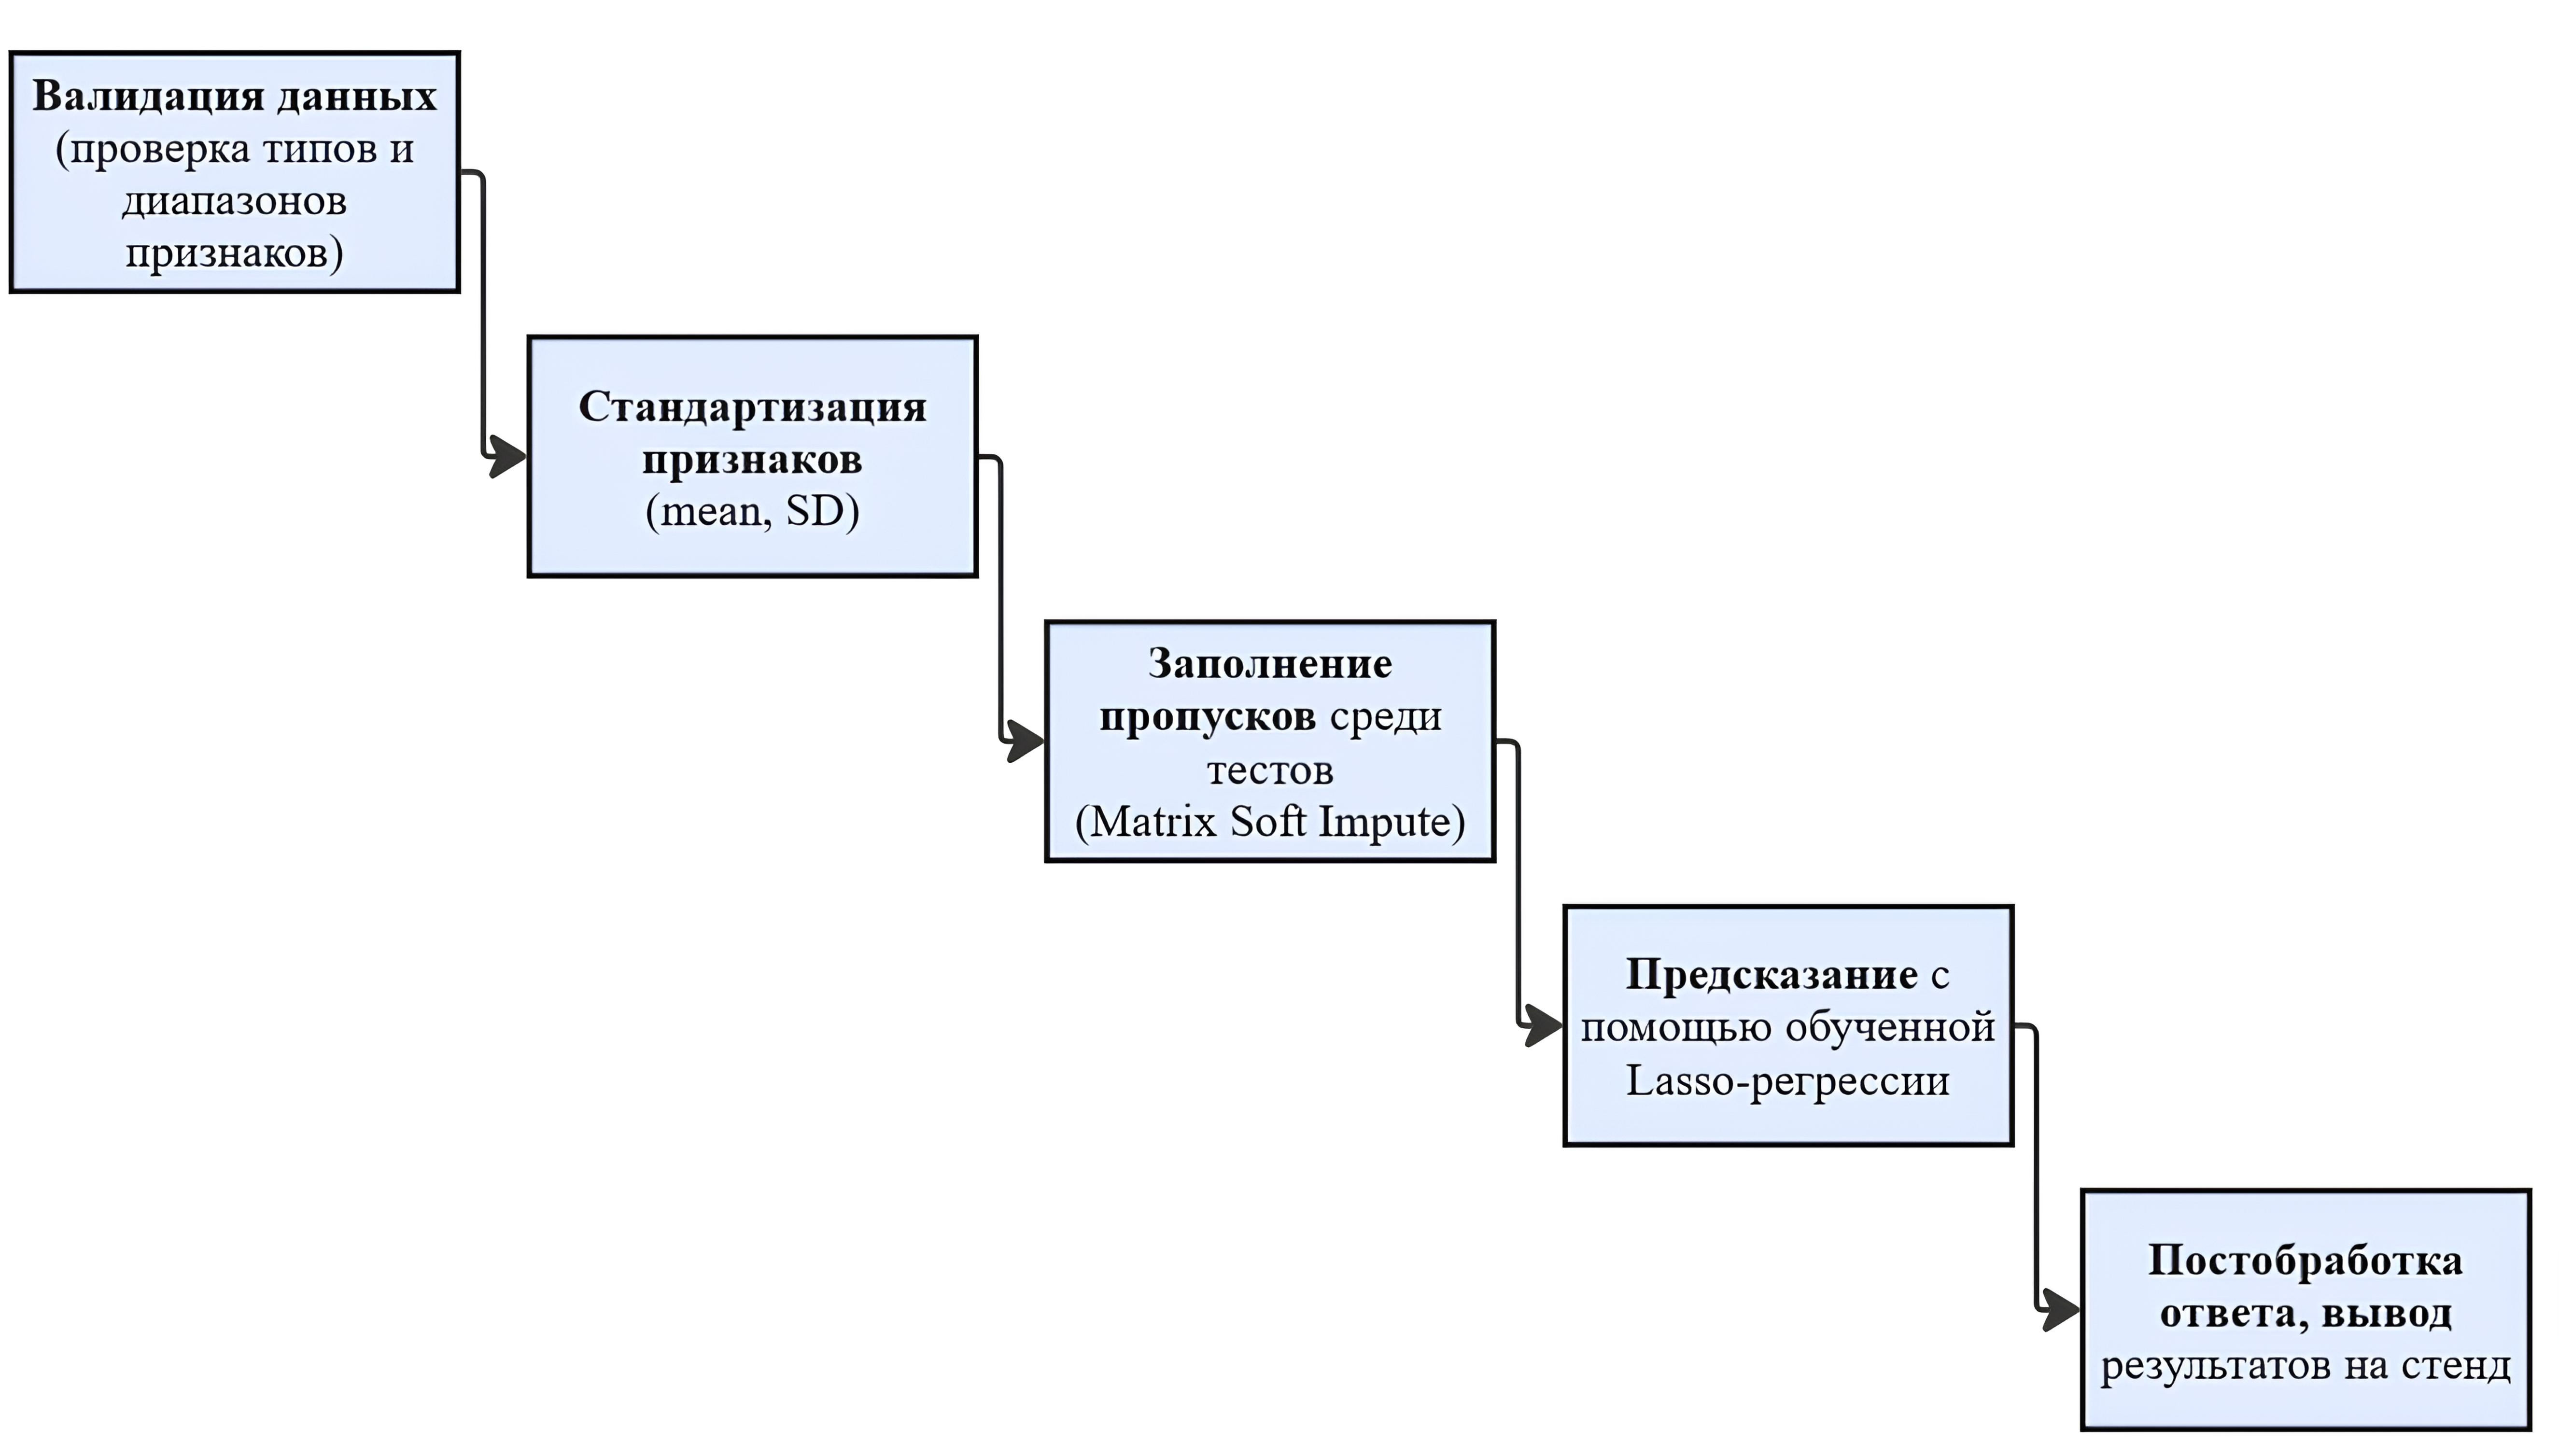
\includegraphics[width=0.85\linewidth]{images/Итоговый пайплайн_ups.jpg}
        \caption{Итоговая последовательность вычислительных этапов для определения кода Голланда по психометрическим тестам при неполных данных}
        \label{fig:pipeline}
    \end{figure}
\end{frame}


% \begin{frame}{Итоговая последовательность вычислительных этапов}
%     \begin{figure}[ht]
%       \centering
%       \begin{tikzpicture}[
%         node distance= -1mm and 4mm,
%         block/.style = {
%           rectangle, draw, fill=cyan!40!blue!5,
%           text width=1.75cm, align=center,
%           rounded corners, minimum height=1.3cm,
%           font=\fontsize{6pt}{7pt}\selectfont
%         },
%         arr/.style = {-{Stealth}, line width=0.8pt}
%       ]
%         % Каскадное расположение практически вплотную
%         \node[block] (b1) {%
%           \textbf{Валидация данных}\\
%           (проверка типов и диапазонов)
%         };
%         \node[block, below right=of b1] (b2) {%
%           \textbf{Стандартизация признаков}\\
%           (mean, SD)
%         };
%         \node[block, below right=of b2] (b3) {%
%           \textbf{Заполнение пропусков среди тестов}\\
%           (Matrix Soft Impute)
%         };
%         \node[block, below right=of b3] (b4) {%
%           \textbf{Предсказание}\\
%           с помощью Lasso-регрессии
%         };
%         \node[block, below right=of b4] (b5) {%
%           \textbf{Постобработка и вывод}\\
%           результатов на стенд
%         };
    
%         % Стрелки с прямыми углами
%         \draw[arr] (b1.east) -- ++(1mm,0) |- (b2.west);
%         \draw[arr] (b2.east) -- ++(1mm,0) |- (b3.west);
%         \draw[arr] (b3.east) -- ++(1mm,0) |- (b4.west);
%         \draw[arr] (b4.east) -- ++(1mm,0) |- (b5.west);
%       \end{tikzpicture}
%     \caption{Итоговая последовательность вычислительных этапов для определения кодов Голланда по психометрическим тестам при неполных данных}
%     \label{fig:data-pipeline}
%     \end{figure}
% \end{frame}


\begin{frame}{Демонстрация прототипа инструмента}
    \begin{figure}
        \centering
        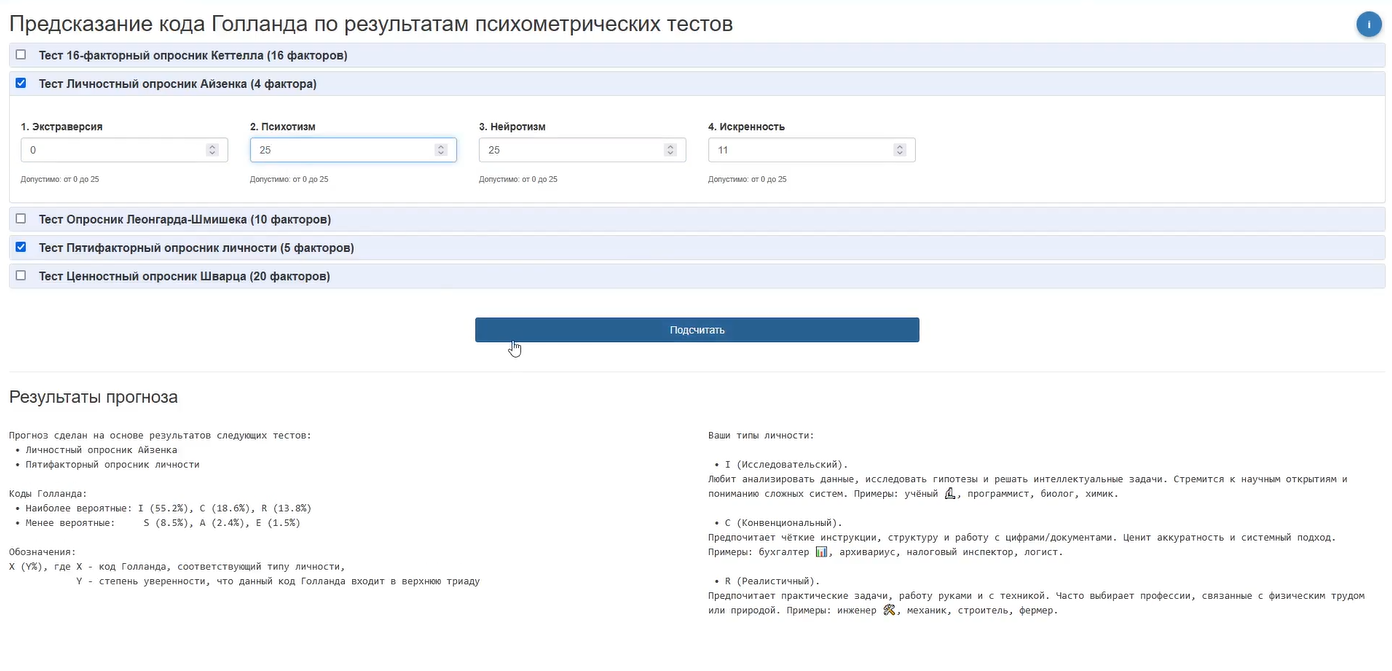
\includegraphics[width=0.95\linewidth]{images/UI1.png}
        \caption{Демонстрация стенда}
        \label{fig:ui1}
    \end{figure}
\end{frame}


\begin{frame}{Демонстрация прототипа инструмента [2]}
    \begin{figure}
        \centering
        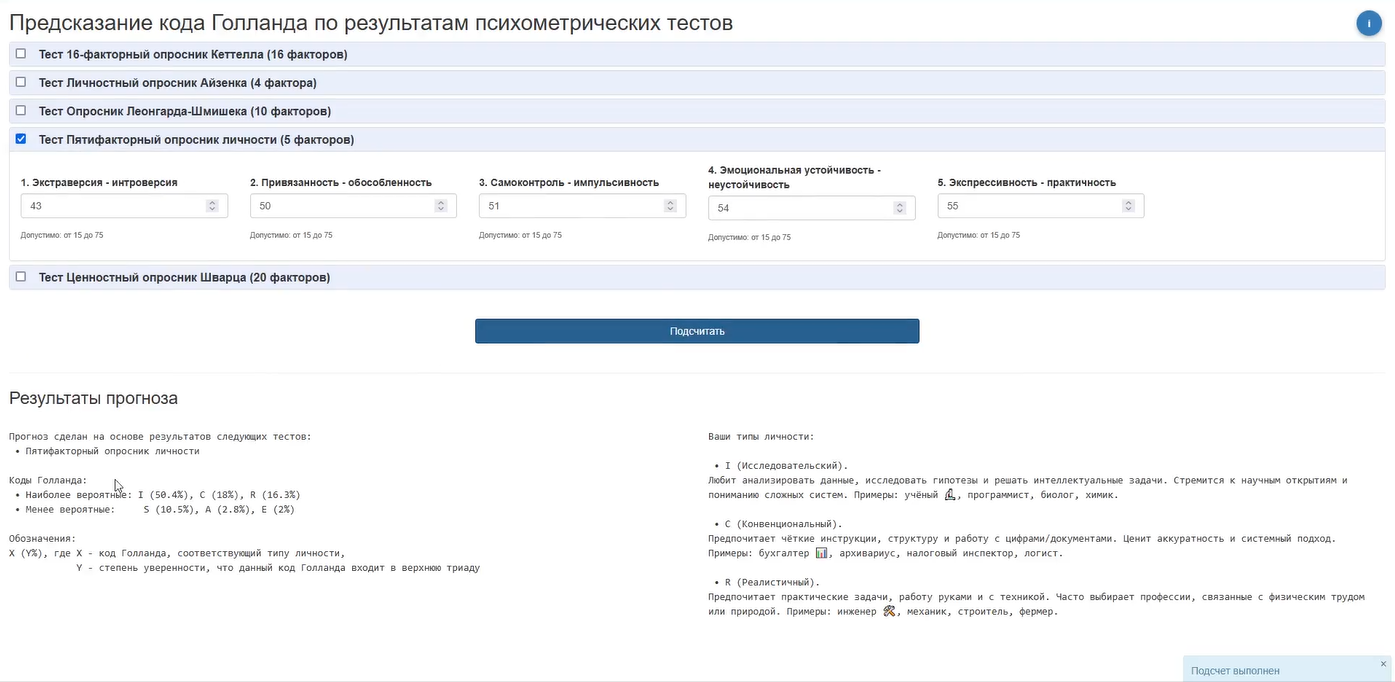
\includegraphics[width=0.95\linewidth]{images/UI2.png}
        \caption{Демонстрация стенда [2]}
        \label{fig:ui2}
    \end{figure}
\end{frame}


\begin{frame}{Результаты}
  \begin{enumerate}
    \item Изучены существующие подходы к определению кода Голланда, поставлены задачи:
      \begin{itemize}
        \item регрессии (multioutput, chain)
        \item классификации (multiclass, multilabel, label powerset)
        \item линейного блендинга базовых моделей
        \item ранжирования
      \end{itemize}
    \item Реализованы модели для предсказания кодов Голланда: лучшие результаты у моделей линейного блендинга на основе метода роя частиц (C‑индекс):
      \begin{itemize}
        \item Ансамбль multioutput‑регрессоров: Lasso-регрессия, пошаговая регрессия, CatBoost, ExtraTrees (11.663)
        \item Ансамбль multilabel‑классификаторов: kNN, SVM, логистическая Lasso-регрессия, XGBoost, LightGBM и др. (11.625)
        \item Показано преимущество «классических» методов перед нейросетевыми
      \end{itemize}
    \item Реализованы алгоритмы восстановления результатов психометрических тестов: лучший – метод мягкой импутации в сочетании с Lasso-регрессией (10.09)
    \item Создан прототип инструмента для определения профориентационных предпочтений: стенд на основе R Shiny
  \end{enumerate}
\end{frame}


\setbeamertemplate{footline}{}
\begin{frame}[plain]
    \titlepage
\end{frame}

\end{document}
